\documentclass[11pt]{article}

% ========================
%        PACKAGES
% ========================
\usepackage{amsmath, amssymb, amsthm}
\usepackage{hyperref}
\usepackage{url}
\usepackage{graphicx}
\usepackage{enumitem}
\usepackage{tikz}
\usetikzlibrary{arrows.meta,shapes.geometric}

% Page layout settings per instructor feedback
\setlength{\textwidth}{17.0cm}
\setlength{\textheight}{24.0cm}
\setlength{\oddsidemargin}{-0.5cm}
\setlength{\evensidemargin}{-0.5cm}
\setlength{\topmargin}{-2.0cm}

% ========================
%      THEOREM STYLES
% ========================
\newtheorem{theorem}{Theorem}[section]
\newtheorem{lemma}[theorem]{Lemma}
\newtheorem{proposition}[theorem]{Proposition}
\newtheorem{corollary}[theorem]{Corollary}

\theoremstyle{definition}
\newtheorem{definition}[theorem]{Definition}

\theoremstyle{remark}
\newtheorem*{remark}{Remark}

% ========================
%      TITLE / AUTHOR
% ========================
\title{Geodesics, Curvature, and Divergence on Finite 2--Manifolds}
\author{Shreshth Rajan}
\date{\today}

\begin{document}

\maketitle

\begin{abstract}
For finite triangulated surfaces, shortest paths carry important geometric information: on spheres, they tend to cluster, while on a torus or projective plane they spread in a qualitatively different way. The growth of small geodesic circles reflects how curvature influences distances in smooth and polyhedral geometry. Here, we observe that curvature appears directly in a circle-length expansion. When we look in the discrete setting, however, this information has to be recovered from only combinatorial data. In this paper, we examine how this recovery works for finite $2$-manifolds in the sense of Knill's discrete differential geometry. We look at several graph $2$--manifolds - here each curvature is encoded by a vertex degree and satisfies a discrete Gauss-Bonnet Identity. In the polyhedral setting, curvature appears as angle defect and controls the exact linear growth of geodesic circles. We use a flat hexagonal tiling as a reference, and discuss a deviation in the growth of graph spheres that measures how far a local metric neighborhood moves from a flat case. At radius 1, this deviation coincides directly with the degree curvature. When summed over all vertices, it gives an exact formula for the Euler characteristic. We compute this functional on standard triangulations of a sphere, torus, and projective plane and find that this quantity tracks the local focusing or spread of shortest paths while also being constrained by the general global topology. In this sense, the growth of graph spheres is a discrete analog of geodesic deviation on finite surfaces. 

\end{abstract}


% ========================
%      SECTION 1
% ========================
\section{Introduction}

A recurring idea in differential geometry is that curvature is not a static invariant of a surface; rather, it actively governs motion. On a smooth surface, the Jacobi equation for geodesic deviation makes this precise: proximal geodesics focus or spread apart based on the sign of the Gaussian curvature. Positive curvature makes geodesics converge, while negative curvature creates divergence. The Gauss-Bonnet theorem makes this local behavior a global statement by relating total curvature to the Euler Characteristic. 

In physical geometry like general relativity, this idea exists in higher dimensions. Curvature ultimately governs how families of geodesics focus or defocus. The less clear part of this, however, is how much of this persists in purely discrete settings. 

This paper addresses this by exploring the following question: \emph{what is the right discrete version of geodesic behavior that reflects curvature on the finite $2$--manifolds we explored?}

We consider two closely related discrete models. The first is purely combinatorial: graph $2$ - manifolds, where geodesics are shortest paths in the graph metric and
metric spheres are defined by graph distance.  The second is geometric: polyhedral (piecewise flat) surfaces, where curvature appears as angle defect at vertices and geodesics are defined using the intrinsic metric.

In this vein, the polyhedral setting provides an interesting guide. Near a vertex $p$, a polyhedral surface is locally isometric to a Euclidean cone with total angle
\[
\Theta(p)=2\pi-K(p).
\]

Here, a direct computation shows that a geodesic circle of radius $r$
has length
\[
L(p,r)=\Theta(p)\,r,
\qquad
L(p,r)-2\pi r=-K(p)\,r.
\]
Therefore, at a cone point, curvature controls geodesic behavior in an explicit way: positive curvature shortens circles and causes geodesics to focus; negative curvature lengthens circles and spreads them apart. 

This observation suggests a discrete analogue. In a graph
$2$ - manifold, the flat reference model is the hexagonal tiling, where the sphere of radius $r$ contains exactly $6r$ vertices.  For a general graph $2$ - manifold $G$ and vertex $v$, we therefore define a divergence functional by
\[
D_G(v,r)=|S_r(v)|-6r,
\]
where $S_r(v)$ denotes the graph sphere of radius $r$.  The first check is clear:
\[
D_G(v,1)=\deg(v)-6=-6K_G(v).
\]
Summing over all vertices yields
\[
\sum_v D_G(v,1)=-6\chi(G),
\]
This shows that the average divergence already encodes global topology.  In this sense, the growth of small metric spheres in the graph setting plays the same role that geodesic circles play in the smooth and polyhedral theories.

The remainder of the paper develops this analogy systematically. Section~2 reviews graph $2$ - manifolds, degree curvature, and the discrete Gauss--Bonnet theorem. Section~3 studies polyhedral surfaces, geodesics, and geodesic fans. Section~4 introduces circle growth and fan behavior in both settings. Section~5 defines the discrete divergence functional and proves its basic
properties.  Section~6 computes the functional on standard triangulated examples.  Section~7 interprets divergence as a discrete analogue of geodesic deviation and discusses possible extensions.

\section{Discrete 2--Manifolds and Curvature in the Graph Setting}

In this section, we recall the discrete $2$-manifold framework from Knill's discrete differential geometry. We discuss a combinatorial curvature that underlies the graph-theoretic Gauss-Bonnet theorem. The goal here is twofold: (i) provide a precise definition of a finite $2$-manifold in this framework and (ii) justify the curvature formula 

\[
K(v) \;=\; 1 - \frac{\deg(v)}{6},
\]
both by a geometric interpretation (ie. angle defect) and by a purely combinatorial Gauss-Bonnet identity.  This is the discrete analogue of the smooth relation between Gaussian curvature and geodesic behavior. We later will use this as a baseline for comparing with a discrete geodesic divergence functional. 

\subsection{Graph 2--Manifolds}

Let $G=(V,E)$ be a finite simple graph.  
For a vertex $v\in V$, the \emph{unit sphere} (or link) of $v$ is the induced subgraph
\[
S(v) := G[\{u \in V : \{u,v\}\in E\}].
\]
Following Knill \cite{KnillGraphGB,KnillMath136Notes}, we call $G$ a \emph{graph $2$--manifold} if each $S(v)$ is a cycle graph $C_n$ with $n\ge 3$, and $G$ admits a triangulation: there exists a collection $F$ of $3$ - element subsets of $V$ such that $(V,E,F)$ is a closed $2$ - dimensional simplicial complex where every face is a triangle and every edge is contained in exactly two faces.  
The Euler characteristic of $G$ is
\[
\chi(G) \;=\; |V| - |E| + |F|.
\]

The cycle condition for $S(v)$ encodes the local manifold requirement that a small neighborhood of $v$ has the topology of a $1$--sphere. This class includes all closed triangulated surfaces: spheres, tori, projective planes, and higher-genus surfaces.

\subsection{Angle Defect and Curvature}

When a graph $2$-manifold is a polyhedral surface in $\mathbb{R}^3$ with each face a Euclidean triangle, curvature is concentrated at vertices.  

If $\sigma \in F$ is a face incident to $v$ and $\theta_\sigma(v)$ is the interior angle of $\sigma$ at $v$, the \emph{angle sum} at $v$ is
\[
\Theta(v) := \sum_{\sigma\ni v} \theta_\sigma(v),
\]
and the \emph{angle-defect curvature} (in class, we called this the \emph{excess angle} \cite{KnillMath136Notes}) is
\[
K_{\mathrm{ang}}(v) := 2\pi - \Theta(v).
\]
Flat Euclidean geometry would contribute a total angle of $2\pi$ around each point, so
$K_{\mathrm{ang}}(v)$ measures the local excess or deficit in curvature.  

The  polyhedral Gauss-Bonnet theorem (e.g., \cite{BobenkoSurisDDG} or the polyhedral curvature discussion from class \cite{KnillMath136Notes}) states that for a closed polyhedral surface,
\[
\sum_{v\in V} K_{\mathrm{ang}}(v) 
\;=\; 2\pi \chi(G).
\]
When all faces are equilateral triangles, each contributes an angle of $\pi/3$. A vertex of degree $d$ then satisfies
\[
\Theta(v) = d \cdot \frac{\pi}{3},
\qquad
K_{\mathrm{ang}}(v) 
= 2\pi - d\cdot \frac{\pi}{3}
= 2\pi\left(1 - \frac{d}{6}\right).
\]
This motivates the normalized \emph{degree curvature}
\[
K_{\mathrm{deg}}(v) := 1 - \frac{\deg(v)}{6},
\]
which coincides with $K_{\mathrm{ang}}(v)/(2\pi)$ for equilateral triangulation.

Thus $K_{\mathrm{deg}}(v)$ is the total curvature (in $2\pi$) from vertex $v$, and serves as a discrete Gaussian curvature.  
This notion appears in several perspectives on discrete curvature, including Forman's combinatorial Ricci curvature \cite{FormanCombinatorialRicci} and  Ollivier's coarse Ricci curvature \cite{OllivierRicci}, though in a different analytic form.

\subsection{Combinatorial Gauss--Bonnet}

An interesting aspect of degree curvature is that it satisfies an exact Gauss-Bonnet identity purely at the graph level. It requires neither an embedding nor metric data.  The following proof from class appears in several texts \cite{KnillGraphGB,KnillMath136Notes}.

\begin{theorem}[Discrete Gauss--Bonnet]
Let $(V,E,F)$ be a closed triangulated graph $2$--manifold.  
Then
\[
\sum_{v\in V} \left(1 - \frac{\deg(v)}{6}\right)
\;=\;
|V| - |E| + |F|
\;=\;
\chi(G).
\]
\end{theorem}

\begin{proof}
Each edge contributes to the degrees of exactly two vertices. Therefore, 
\[
\sum_{v\in V} \deg(v) = 2|E|.
\]
Thus
\[
\sum_{v\in V} \left(1 - \frac{\deg(v)}{6}\right)
= |V| - \frac{1}{6}\sum_{v\in V}\deg(v)
= |V| - \frac{1}{3}|E|.
\]
Each face has three edges. Each edge is contained in precisely two faces (ie. the surface has no boundary), so $3|F| = 2|E|$ and hence $|E| = \tfrac{3}{2}|F|$.  
Substituting,
\[
|V| - \frac{1}{3}|E|
= |V| - \frac{1}{3}\cdot \frac{3}{2}|F|
= |V| - \frac{1}{2}|F|
= |V| - |E| + |F|
=
\chi(G).
\]
\end{proof}

This  combinatorial theorem is the discrete analogue of the smooth Gauss-Bonnet formula familiar from classical differential geometry  (see, e.g., \cite{doCarmoCurvesSurfaces,ONeillElementaryDG,SpivakCIDG2}).  
When the triangulation is equilateral, it is also equivalent to the polyhedral
Gauss-Bonnet theorem. This is because of $K_{\mathrm{ang}}(v) = 2\pi K_{\mathrm{deg}}(v)$.

\subsection{Examples: Sphere, Torus, Projective Plane}

Here, we note three standard triangulations for later reference.

\paragraph{Sphere (tetrahedron).}
Here $|V|=4$, $|E|=6$, $|F|=4$, so $\chi=2$.  
Each vertex has degree $3$, hence $K(v)=1/2$ and 
$\sum_v K(v)=2=\chi$.

\paragraph{Torus.}
A studied minimal triangulation has $|V|=7$, $|E|=21$, $|F|=14$,  resulting in $\chi=0$.  
Every vertex has degree $6$, so $K(v)=0$ for all $v$ and  $\sum_v K(v)=0=\chi$.

\paragraph{Projective plane.}
A classical triangulation has $|V|=6$, $|E|=15$, $|F|=10$, giving $\chi=1$.  Every vertex has degree $5$, so $K(v)=1/6$, and $\sum_v K(v)=1=\chi$.

These examples show three canonical curvature regimes: strictly positive, identically zero, and somewhat positive total curvature. Later in the paper, these serve as benchmark geometries when we study geodesic spreading and the discrete
divergence functional. 

\begin{figure}[ht]
\centering
\begin{tikzpicture}[scale=1.2]
% Positive curvature: deg = 5
\begin{scope}[xshift=-4cm]
\node[circle,fill=black,inner sep=2pt] (v1) at (0,0) {};
\foreach \i in {1,...,5} {
  \node[circle,fill=blue,inner sep=1.5pt] (n1\i) at ({72*\i-90}:1) {};
  \draw (v1) -- (n1\i);
}
\draw[-] (n11) -- (n12) -- (n13) -- (n14) -- (n15) -- (n11);
\node[below] at (0,-1.5) {$\deg(v)=5$};
\node[below] at (0,-1.9) {$K_G(v)=\frac{1}{6}>0$};
\end{scope}

% Flat: deg = 6 (hexagonal)
\begin{scope}
\node[circle,fill=black,inner sep=2pt] (v2) at (0,0) {};
\foreach \i in {1,...,6} {
  \node[circle,fill=green!60!black,inner sep=1.5pt] (n2\i) at ({60*\i-90}:1) {};
  \draw (v2) -- (n2\i);
}
\draw[-] (n21) -- (n22) -- (n23) -- (n24) -- (n25) -- (n26) -- (n21);
\node[below] at (0,-1.5) {$\deg(v)=6$};
\node[below] at (0,-1.9) {$K_G(v)=0$ (flat)};
\end{scope}

% Negative curvature: deg = 7
\begin{scope}[xshift=4cm]
\node[circle,fill=black,inner sep=2pt] (v3) at (0,0) {};
\foreach \i in {1,...,7} {
  \node[circle,fill=red,inner sep=1.5pt] (n3\i) at ({360/7*\i-90}:1) {};
  \draw (v3) -- (n3\i);
}
\draw[-] (n31) -- (n32) -- (n33) -- (n34) -- (n35) -- (n36) -- (n37) -- (n31);
\node[below] at (0,-1.5) {$\deg(v)=7$};
\node[below] at (0,-1.9) {$K_G(v)=-\frac{1}{6}<0$};
\end{scope}
\end{tikzpicture}
\caption{Curvature regimes on graph 2-manifolds. Left: positive curvature (degree 5). Center: flat (degree 6, hexagonal). Right: negative curvature (degree 7). The unit sphere $S_1(v)$ forms a cycle around the central vertex.}
\label{fig:curvature-regimes}
\end{figure}

\section{Polyhedral Surfaces, Geodesics, and Geodesic Fans}
\label{sec:polyhedral}

In the last section, we worked in the combinatorial space of graph $2$ manifolds and degree curvature. Here, we move into the polyhedral world. Geodesics and geodesic ''fans'' can be defined in the metric sense, with curvature being an angle defect at vertices. The aim is to make more precise Knill's comment \cite{KnillGraphGB,KnillMath136Notes}: in regions of positive curvature, geodesic fans focus and small circles are shorter than in the flat plane. In regions of negative curvature, fans spread and circles are longer. This provides the geometric intuition that our later discrete divergence functional is designed to capture combinatorially.

\subsection{Polyhedral Surfaces and the Intrinsic Metric}

Let $(V,E,F)$ be a closed triangulated graph $2$-manifold.  A \emph{polyhedral realization} (also called a \emph{geometric realization}) of this triangulation is a map $\iota:V\to\mathbb{R}^3$ s.t. for each face $\sigma=\{v_1,v_2,v_3\}\in F$, the points $\iota(v_1),\iota(v_2),\iota(v_3)$ are non-collinear and span a Euclidean triangle, and distinct faces intersect only in
common edges, common vertices, or not at all.  The resulting set
\[
M := \bigcup_{\sigma\in F} \triangle(\iota(\sigma)) \subset \mathbb{R}^3
\]
is a piecewise-flat polyhedral surface \cite{BobenkoSurisDDG}.

The \emph{intrinsic distance} $d_M(x,y)$ between points $x,y\in M$ is defined as the infimum of Euclidean lengths of rectifiable curves on $M$ joining $x$ to $y$.  Equipped with this length metric, $(M,d_M)$ is a geodesic metric space: for sufficiently close points, there exist shortest paths realizing the distance (see, e.g., \cite{BobenkoSurisDDG}).

A curve $\gamma:I\to M$ (with $I\subset\mathbb{R}$ an interval) is a \emph{geodesic} if, locally, it is length minimizing: each point of $\gamma$ has a neighborhood on which
$\gamma$ realizes the intrinsic distance between its endpoints.

\subsection{Geodesics on Triangle Meshes}

The structure of geodesics on polyhedral surfaces is particularly simple away from
vertices. Inside the interior of a single face, the metric is just the restriction of
the Euclidean metric on a triangle.

\begin{lemma}
Let $\gamma:[a,b]\to M$ be a geodesic whose image on $[a,b]$ lies in the interior of a single triangular face.  Then $\gamma([a,b])$ is a straight line segment in that triangle.
\end{lemma}

\begin{proof}[Proof sketch]
In the interior of a face, the induced metric is Euclidean.  Any locally length-minimizing curve in a Euclidean domain is a straight segment: if $\gamma$ were not straight, we could replace the arc between $\gamma(a)$ and $\gamma(b)$ by the straight segment joining these endpoints inside the face, strictly shortening its length, contradicting local minimality.
\end{proof}

When a geodesic crosses an edge between two adjacent faces, it remains straight after \emph{unfolding} the faces into the plane.

\begin{lemma}
Let $\gamma$ be a geodesic that crosses an edge $e$ at a point $p$ which is not a vertex.  Suppose $e$ is shared by two faces $\sigma_1$ and $\sigma_2$.  If we develop $\sigma_1$ and $\sigma_2$ isometrically into the Euclidean plane by reflecting one triangle across $e$, then the image of $\gamma$ in this unfolded configuration is a straight line near $p$.
\end{lemma}

\begin{proof}[Proof sketch]
Take a small neighborhood of $p$ in $\sigma_1\cup\sigma_2$. Unfold the two triangles along $e$ into a single  quadrilateral.  The unfolded metric is Euclidean, so a locally length-minimizing curve in this patch must be a straight segment.  Folding back identifies the two copies of $e$ and shows that $\gamma$ crosses the edge with no corner when viewed in a fully developed plane; if there were a corner, it could be smoothed and the curve could be shortened, which contradicts minimality.  This is the standard unfolding argument for polyhedral geodesics \cite{BobenkoSurisDDG}.
\end{proof}

At any vertex, the metric is singular: curvature is concentrated. Geodesics can branch or have non-unique continuations. We further explore geodesics from a vertex and the behavior of small circles around it by modeling vertex neighborhoods as Euclidean cones. 

\subsection{Vertex Cones and Small Geodesic Circles}

Let $v\in V$ be a vertex of the triangulation.  Denote by $\sigma_1,\dots,\sigma_k$ the faces incident to $v$, and let $\theta_i(v)\in(0,\pi)$ be the interior angle at $v$ in the face $\sigma_i$.  The total angle around $v$ is
\[
\Theta(v) := \sum_{i=1}^k \theta_i(v),
\]
and the angle-defect curvature is $K_{\mathrm{ang}}(v) = 2\pi - \Theta(v)$, as in Section~2.

The local geometry of $M$ near $v$ is modeled by a Euclidean cone.  For $\alpha>0$, the \emph{Euclidean cone} $C_\alpha$ is obtained from the planar sector
\[
S_\alpha = \{(r,\varphi) : r\ge 0,\ 0\le \varphi < \alpha\}
\]
with metric $dr^2 + r^2 d\varphi^2$ by identifying the boundary rays $\varphi=0$ and $\varphi=\alpha$; see \cite{BobenkoSurisDDG} for a standard reference.

\begin{proposition}\label{prop:cone-isometry}
For sufficiently small $\varepsilon>0$, the intrinsic metric on the star
\[
\mathrm{Star}_\varepsilon(v) := \{ x\in M : d_M(x,v) < \varepsilon \}
\]
is isometric to a neighborhood of the tip in the Euclidean cone $C_{\Theta(v)}$. In particular, the total angle around $v$ in the intrinsic metric is $\Theta(v)$, and the curvature concentrated at $v$ is $K_{\mathrm{ang}}(v)=2\pi-\Theta(v)$.
\end{proposition}

\begin{proof}[Proof idea]
Unfold the faces $\sigma_1,\dots,\sigma_k$ around $v$ into the plane by successively gluing along the edges that meet at $v$, preserving edge lengths.  The union of the unfolded triangles is a planar sector of angle $\Theta(v)$.  Identifying the two boundary rays produces a cone of angle $\Theta(v)$, and the induced metric coincides with the intrinsic metric on a sufficiently small neighborhood of $v$ in $M$
\cite{BobenkoSurisDDG}.
\end{proof}

In the cone $C_\alpha$, circles centered at the tip have circumference proportional to the cone angle.

\begin{lemma}
Let $C_\alpha$ be the Euclidean cone of angle $\alpha$.  The geodesic circle of radius $r>0$ centered at the tip has intrinsic length $L_\alpha(r) = \alpha r$.
\end{lemma}

\begin{proof}
In the sector model $S_\alpha$, the circle of radius $r$ is parameterized by $\varphi\in[0,\alpha)$ with line element $ds = r\, d\varphi$.  Integrating gives $L_\alpha(r) = \int_0^\alpha r\, d\varphi = \alpha r$, which descends to the cone after identifying the boundary rays.
\end{proof}

Now, with $\alpha=\Theta(v)$, we get: 

\begin{corollary}
For sufficiently small $r>0$, the intrinsic geodesic circle
\[
C_r(v) := \{ x\in M : d_M(x,v) = r \}
\]
has length
\[
L(v,r) = \Theta(v)\, r = (2\pi - K_{\mathrm{ang}}(v))\, r.
\]
Equivalently,
\[
L(v,r) - 2\pi r = -K_{\mathrm{ang}}(v)\, r.
\]
\end{corollary}

\begin{figure}[ht]
\centering
\begin{tikzpicture}[scale=1.1]
% Draw cone surface
\fill[black!8] (0,0) -- (-2.2,-3.5) arc (180:360:2.2 and 0.65) -- cycle;
\draw[thick] (0,0) -- (-2.2,-3.5);
\draw[thick] (0,0) -- (2.2,-3.5);
\draw[thick,dashed] (-2.2,-3.5) arc (180:360:2.2 and 0.65);

% Draw geodesic circle at radius r
\draw[very thick,blue] (-1.5,-2.4) arc (180:360:1.5 and 0.45);
\draw[very thick,blue,dashed] (-1.5,-2.4) arc (180:0:1.5 and 0.45);

% Labels
\node[above] at (0,0.2) {vertex $p$};
\draw[<->,thick] (0.1,-0.05) -- (1.5,-2.35) node[midway,right,xshift=2pt] {$r$};
\node[blue,right] at (1.7,-2.2) {$C_r(p)$};

% Angle annotation
\node[left,align=right] at (-2.6,-2.0) {cone angle\\$\Theta(p)$};
\draw[->,thick] (-2.4,-2.2) -- (-1.8,-2.8);

\end{tikzpicture}

\vspace{0.3cm}
\noindent Key relations: $\Theta(p) = 2\pi - K(p)$, \quad $L(p,r) = \Theta(p) \cdot r$, \quad $L(p,r) - 2\pi r = -K(p) \cdot r$

\caption{Geodesic circle on a polyhedral cone. A neighborhood of a vertex with angle defect $K(p)$ is isometric to a Euclidean cone of angle $\Theta(p)=2\pi-K(p)$. The geodesic circle at radius $r$ has length $L(p,r)=\Theta(p) r$, giving first-order deviation proportional to curvature.}
\label{fig:cone-circle}
\end{figure}

\subsection{Geodesic Fans and Curvature}

We now formalize the ``fan'' picture. Fix a vertex $v$ and consider geodesic rays emanating from $v$ in different directions.

\begin{definition}
A \emph{geodesic ray} from $v$ is a unit--speed geodesic $\gamma:[0,\infty)\to M$ with $\gamma(0)=v$. In the cone model $C_{\Theta(v)}$, such a ray corresponds to a straight ray from the tip with some initial direction angle $\varphi_0$.
\end{definition}

\begin{definition}
A \emph{geodesic fan} of width $\Delta\varphi>0$ from $v$ is a one-parameter family $\{\gamma_\varphi\}_{\varphi\in[\varphi_0,\varphi_0+\Delta\varphi]}$ of geodesic rays from $v$ whose initial directions in the cone $C_{\Theta(v)}$ fill the angular sector $[\varphi_0,\varphi_0+\Delta\varphi]$.
\end{definition}

At radius $r>0$, the points $\gamma_\varphi(r)$ lie on the circle $C_r(v)$ and form an arc of length
\[
\ell(r) = r\Delta\varphi,
\]
since the line element along $C_r(v)$ in the cone model is $ds = r\, d\varphi$.  For a fixed number $N$ of equally spaced rays filling out a full circle, the average spacing between neighboring rays at radius $r$ is proportional to
\[
\frac{L(v,r)}{N} = \frac{\Theta(v) r}{N}.
\]
Compared to the flat case, where $\Theta = 2\pi$, we see:

\begin{itemize}
  \item If $K_{\mathrm{ang}}(v)>0$ (so $\Theta(v)<2\pi$), then $L(v,r)<2\pi r$ and
        geodesic fans are ``compressed'': the same number of rays occupy a shorter
        circle, and neighboring geodesics remain closer.
  \item If $K_{\mathrm{ang}}(v)<0$ (so $\Theta(v)>2\pi$), then $L(v,r)>2\pi r$ and
        geodesic fans are ``expanded'': rays spread further apart than in the flat
        model.
\end{itemize}

This relationship between curvature and the size of small circles is the polyhedral analogue of geodesic deviation in the smooth setting.. It is exactly the behavior our discrete divergence functional will measure in the combinatorial world (compare, for instance, with the smooth treatment in \cite{doCarmoCurvesSurfaces,ONeillElementaryDG,SpivakCIDG2}).

\subsection{Smooth Puiseux Expansion and Discrete Analogue}

On a smooth Riemannian surface, the length $L(r)$ of the geodesic circle of radius $r$ around a point $p$ with Gaussian curvature $K(p)$ admits the classical small radius expansion
\[
L(r) = 2\pi r - \frac{K(p)}{3}\, r^3 + O(r^5),
\]
see, for example, \cite{doCarmoCurvesSurfaces,ONeillElementaryDG,SpivakCIDG2}.  
The leading term $2\pi r$ is the Euclidean circumference, and the sign of $K(p)$ determines whether $L(r)$ is shorter or longer than the flat value at order $r^3$. Positive curvature causes geodesics to focus, negative curvature makes them diverge.

\section{Geodesic Fans and Local Divergence}
\label{sec:fan-growth}

In the previous section we described geodesics on polyhedral surfaces through their intrinsic metric and the unfolding rule across edges \cite{BobenkoSurisDDG}. We now examine how families of such geodesics (`''geodesic fans'') encode the local curvature of the surface.  Here, we provide the geometric foundation for the discrete divergence functional discussed later.  Throughout, $M$ is a polyhedral surface with its intrinsic length metric, and $p\in M$ is a fixed vertex with angle defect $K(p)=2\pi-\Theta(p)$, per the cone model for polyhedral vertices \cite{BobenkoSurisDDG}.

\subsection{Geodesic rays and angular structure}

By Proposition~\ref{prop:cone-isometry}, a sufficiently small intrinsic neighborhood of $p$ is isometric to a Euclidean cone $C_{\Theta(p)}$ of total angle $\Theta(p)$ \cite{BobenkoSurisDDG}.  In this model, each geodesic ray from $p$ corresponds to a straight ray with polar coordinates $(r,\varphi)$, where $\varphi\in[0,\Theta(p))$ is an angular parameter intrinsic to the cone.  Thus the space of initial geodesic directions at $p$ has total angular measure $\Theta(p)$ rather than $2\pi$. Positive curvature ($K(p)>0$) reduces the local angular space; negative curvature increases it.

Let $\gamma_{\varphi}(r)=(r,\varphi)$ denote the geodesic ray of direction
$\varphi$.  If $\Delta=|\varphi_1-\varphi_2|$ is the angular separation of two
rays, the intrinsic distance between $\gamma_{\varphi_1}(r)$ and
$\gamma_{\varphi_2}(r)$ is, by the Euclidean law of cosines applied in the
developed sector,
\[
d\big(\gamma_{\varphi_1}(r),\gamma_{\varphi_2}(r)\big)
    = 2r\sin\!\left(\frac{\Delta}{2}\right).
\]
For small $\Delta$ we obtain the linear approximation
\[
d\big(\gamma_{\varphi_1}(r),\gamma_{\varphi_2}(r)\big)
    = r\Delta + O(r\Delta^{3}),
\]
showing that geodesic rays separate linearly in $r$.  The coefficient of this
linear term is controlled entirely by the cone angle $\Theta(p)$.

\subsection{Combinatorial analogy: spheres in graph 2-manifolds}

The same phenomenon appears in Knill's discrete 2-manifold graphs
\cite{KnillGraphGB,KnillMath136Notes}.  For a
vertex $v$ of a 2-manifold graph $G$, let $S_r(v)$ denote the sphere of
graph-distance $r$.  In a flat (degree-$6$) region one has $|S_r(v)|=6r$.
The graph curvature
\[
K_G(v)=1-\frac{\deg(v)}{6}
\]
captures deviations from flatness \cite{KnillGraphGB}.  At radius $r=1$,
\[
|S_1(v)|=\deg(v)=6-6K_G(v),
\]
and for small $r$ the shells $S_r(v)$ expand more slowly when $\deg(v)<6$ and
more quickly when $\deg(v)>6$.  Thus the sign of $K_G(v)$ dictates the initial
expansion behavior exactly as in the polyhedral case.

\subsection{Compatibility of the polyhedral and graph models}

The two pictures agree at the level of first-order expansion.  At a polyhedral
vertex with angle defect $K(p)$, the metric circle satisfies
\[
L(p,r) - 2\pi r = -K(p)\,r.
\]
At a vertex of a graph 2-manifold one has, to first order,
\[
|S_r(v)| - 6r = -6 K_G(v) + O(1),
\]
in the flat-hexagonal normalization \cite{KnillGraphGB,KnillMath136Notes}.
Here $L(p,r)$ denotes the continuous length of a geodesic circle on the polyhedral surface, while $|S_r(v)|$ denotes the discrete vertex count in the graph sphere; these are parallel but distinct quantities.
Identifying the flat reference lengths $2\pi r$ and $6r$, the two deviations
match in sign and linear order.  This agreement justifies treating geodesic
fan behavior and combinatorial sphere growth as parallel manifestations of
curvature in finite 2-manifolds and provides the theoretical foundation for the
discrete divergence functional discussed in the next section.

\section{A Discrete Geodesic Divergence Functional}
\label{sec:divergence}

For polyhedral surfaces, sections~\ref{sec:polyhedral}--\ref{sec:fan-growth} showed that the geodesic circle centered at a vertex $p$ satisfies the linear law \cite{BobenkoSurisDDG}
\[
L(p,r)=\Theta(p)\, r = (2\pi - K(p))\, r,
\]
so that the deviation
\[
D_M(p,r) := L(p,r)-2\pi r = -K(p)\, r
\]
encodes the sign and magnitude of curvature at $p$ to first order.  This extends the well-known smooth expansion of geodesic circles \cite{doCarmoCurvesSurfaces,ONeillElementaryDG,SpivakCIDG2}.  

Here, we discuss a \emph{combinatorial} analogue of this ``first-order circle deviation'' for graph $2$-manifolds. This is intrinsic to the graph metric and behaves analogously to the polyhedral model when the curvature is small or localized.  The functional is both
geometrically natural and computationally simple; as in, it depends only on the sizes
of discrete metric spheres.

\subsection{Motivation from circles in the flat and conical metrics}

In the polyhedral setting, the local model near a vertex is a Euclidean cone
with cone angle $\Theta(p)$ \cite{BobenkoSurisDDG}.   The circumference of a radius--$r$ circle grows linearly with $r$, and the difference from the Euclidean law $2\pi r$ is exactly $-K(p)\, r$.  As a result, curvature controls the \emph{first-order divergence or convergence} of geodesic fans.

For graph $2$-manifolds, the natural flat reference is the hexagonal tiling $H$, where every vertex has degree~$6$ and the sphere of radius $r$ has
\[
|S_r^H(v)| = 6r
\quad\text{for all }r\ge1,
\]
a standard fact in discrete differential geometry  
\cite{KnillGraphGB,KnillMath136Notes}.  
This is the combinatorial analogue of $2\pi r$.  Our aim is to measure how $|S_r(v)|$ deviates from $6r$.

\subsection{Definition of the divergence functional}

Let $G=(V,E)$ be a graph $2$-manifold and let $v\in V$.
We write
\[
S_r(v) := \{\, u\in V : d_G(u,v)=r \,\}
\]
for the graph sphere of radius $r\in\mathbb{N}$ (integer distance).  The \emph{discrete divergence functional} is defined by
\[
D_G(v,r) := |S_r(v)| - 6r
\]
for integer $r\ge 1$. Equivalently, a normalized version
\[
\widehat{D}_G(v,r) := \frac{|S_r(v)|}{6r}-1
\]
captures the relative deviation from the flat law. We work primarily with $D_G(v,r)$ since it has cleaner additive properties and aligns directly with the polyhedral formula $L(p,r)-2\pi r$.

\subsection{Basic properties and relation to curvature}

\paragraph{Locality.}
Since $S_r(v)$ depends only on the ball $B_r(v)$, the functional $D_G(v,r)$ is completely local.  As in, any changes to the graph outside $B_r(v)$ do not affect it. This is in parallel to the metric fact that $L(p,r)$ depends only on the geometry in the geodesic ball $B_r(p)$ \cite{BobenkoSurisDDG}.

\paragraph{Flat calibration.}
 Out to radius $r$, if $G$ agrees with a patch of the hexagonal tiling, then $|S_r(v)|=6r$ and hence $D_G(v,r)=0$.  Thus $D_G$ vanishes exactly in the combinatorial flat case, as captured in Knill's curvature framework
\cite{KnillGraphGB}.

\paragraph{First-order behavior at $r=1$.}
At radius $1$ we have $|S_1(v)|=\deg(v)$, so using Knill’s degree curvature
\[
K_G(v) = 1 - \frac{\deg(v)}{6},
\]
\cite{KnillGraphGB}
we obtain the exact identity
\[
D_G(v,1) = \deg(v) - 6 = -6 K_G(v).
\]
As a result, the sign of $D_G(v,1)$ agrees with the sign of $-K_G(v)$. This directly reproduces the metric relation $D_M(p,r) = -K(p)\, r$ when $r=1$.  In particular:
\[
\deg(v)<6 \iff D_G(v,1)<0,\qquad
\deg(v)>6 \iff D_G(v,1)>0.
\]

\paragraph{Behavior for $r>1$.}
As the radii get larger, the value of $D_G(v,r)$ depends on the combinatorics of neighbors-of-neighbors and cannot be reduced to a closed formula. But, as long as curvature is concentrated near $v$, or the degrees in $B_r(v)$ are biased above or below $6$, the sign of $D_G(v,r)$ typically matches the sign of $-K_G(v)$. The deviation reflects the accumulated contribution of curvature in the ball.  Using explicit triangulations of the sphere, torus, and projective plane, section~\ref{sec:examples} shows this behavior. 
\cite{KnillMath136Notes}.

\subsection{Comparison with the polyhedral divergence functional}

Previously, in the metric setting we defined
\[
D_M(p,r) = L(p,r)-2\pi r = -K(p)\, r
\]
for a cone point $p$ \cite{BobenkoSurisDDG}.  
The graph formula
\[
D_G(v,r) = |S_r(v)| - 6r
\]
is the exact combinatorial analogue, with $6$ playing the role of $2\pi$. The identity $D_G(v,1)=-6K_G(v)$ is a discrete version of the metric relation $\frac{\partial}{\partial r}D_M(p,r)|_{r=0} = -K(p)$, showing that the \emph{first-order divergence of geodesic fans} in the graph metric detects the same curvature that appears in the Gauss--Bonnet theorem for graphs 
\cite{KnillGraphGB}.

\section{Examples and Computations}
\label{sec:examples}

Here, we compute the discrete divergence functional on several canonical triangulated surfaces and compare its behavior with the underlying curvature distribution established by the degree curvature $K_G(v)=1-\deg(v)/6$ and the Gauss--Bonnet identity \cite{KnillGraphGB,KnillMath136Notes}.  The examples  illustrate three distinct regimes: globally positive curvature (spherical polyhedra), globally zero curvature (torus), and mixed curvature with positive Euler characteristic (projective plane).  Throughout, we write
\[
D_G(v,r) = |S_r(v)| - 6r,
\qquad
\widehat{D}_G(v,r) = \frac{|S_r(v)|}{6r} - 1,
\]
and recall from Section~\ref{sec:divergence} that
\[
D_G(v,1) = \deg(v)-6 = -6K_G(v).
\]

\subsection{The tetrahedral sphere: uniformly positive curvature}

The tetrahedron is the unique $3$-regular triangulation of $S^2$, with
$(V,E,F)=(4,6,4)$ and Euler characteristic $2$ \cite{KnillMath136Notes}.
Each vertex satisfies
$\deg(v)=3$, hence
\[
K_G(v)=1-\frac{3}{6}=\frac{1}{2},
\qquad
\sum_v K_G(v) = 4 \cdot \frac{1}{2} = 2 = \chi(S^2).
\]
The tetrahedral graph is the complete graph $K_4$, where every vertex is adjacent to every other vertex. The graph metric spheres are:
\[
S_1(v) = \text{three neighbors}, \qquad |S_1(v)|=3,
\]
and $S_2(v)=\varnothing$ (the empty set), since the graph diameter is $1$.
Thus
\[
D_G(v,1) = 3-6 = -3.
\]

\begin{figure}[ht]
\centering
\begin{tikzpicture}[scale=1.3]
% Define vertices of tetrahedron (K_4 complete graph)
\coordinate (v1) at (0,2);
\coordinate (v2) at (-1.5,-0.5);
\coordinate (v3) at (1.5,-0.5);
\coordinate (v4) at (0,-1.8);

% Draw all edges (complete graph)
\draw[thick] (v1) -- (v2) -- (v3) -- (v1);
\draw[thick] (v1) -- (v4);
\draw[thick] (v2) -- (v4);
\draw[thick] (v3) -- (v4);

% Draw vertices
\foreach \v in {v1,v2,v3,v4} {
  \fill[black] (\v) circle (3pt);
}

% Label vertices
\node[above] at (v1) {$v$};
\node[left] at (v2) {$u_1$};
\node[right] at (v3) {$u_2$};
\node[below] at (v4) {$u_3$};

% Highlight S_1(v)
\draw[blue,thick,dashed] (v2) -- (v3) -- (v4) -- (v2);
\node[blue,right] at (1.8,0) {$S_1(v)$};

% Statistics
\node[below,align=left] at (0,-3.2) {
  Complete graph $K_4$: every vertex adjacent to all others\\
  Diameter = 1, \quad $|S_1(v)|=3$, \quad $|S_2(v)|=\varnothing$\\
  $D_G(v,1) = 3-6=-3$ \quad (negative = focusing)
};
\end{tikzpicture}
\caption{The tetrahedral graph $K_4$ (complete graph on 4 vertices). Each vertex has degree 3, giving positive curvature $K_G(v)=1/2$. Since diameter is 1, all vertices lie in $S_1(v)$ and $S_2(v)$ is empty.}
\label{fig:tetrahedron-k4}
\end{figure}

Here, the negative sign reflects the \emph{focusing} of geodesic fans predicted by
positive curvature. Note that for $r\ge 2$, the functional $D_G(v,r)$ is undefined for this graph, as all vertices are at distance at most $1$ from each other.

\subsection{The octahedral sphere: milder positive curvature}

The octahedron has $(V,E,F)=(6,12,8)$ with $\deg(v)=4$ at every vertex
\cite{KnillMath136Notes}:
\[
K_G(v) = 1-\frac{4}{6} = \frac{1}{3},
\qquad
\sum_v K_G(v)=6\cdot \frac{1}{3}=2=\chi(S^2).
\]
A vertex $v$ has four neighbors, hence
\[
D_G(v,1)=4-6=-2.
\]
At radius $2$ the sphere $S_2(v)$ consists of the vertex antipodal to $v$ and
its two adjacent vertices, giving $|S_2(v)|=3$ and
\[
D_G(v,2)=3-12=-9.
\]

Here, the divergence has a smaller magnitude at $r=1$ but remains strongly negative in comparison with the tetrahedron. This matches the fact that $K_G=1/3<1/2$.  Both examples corroborate the linear first-order law $D_G(v,1)=-6K_G(v)$ derived from Knill's curvature framework \cite{KnillGraphGB}.

\subsection{A local hyperbolic patch: negative curvature}

To illustrate negative curvature, consider a vertex $v$ in a triangulated surface for which $\deg(v)=7$.  Then
\[
K_G(v)= 1 - \frac{7}{6} = -\frac{1}{6},
\qquad
D_G(v,1)=7-6=1>0.
\]
The positive value indicates that the first metric sphere grows faster than in the flat reference model.  If the neighbors of $v$ have degrees close to $6$, so that curvature is concentrated near $v$, the second sphere typically satisfies $|S_2(v)| \approx 6\cdot 2 + 1$, giving
\[
D_G(v,2) \approx 13 - 12 = 1>0.
\]
This mirrors the polyhedral situation, in which a vertex of negative angle defect produces $L(p,r) > 2\pi r$, reflecting the divergence of nearby geodesics \cite{BobenkoSurisDDG}.

\subsection{Triangulated tori: curvature cancellation and near-zero divergence}

Every triangulated torus $T^2$ satisfies $\chi(T^2)=0$ and thus
\[
\sum_{v\in V(T^2)} K_G(v) = 0
\]
\cite{KnillGraphGB}.  
Minimal triangulations (e.g.\ the $7$-vertex triangulation) have \emph{every} vertex of degree $6$, so the surface is combinatorially flat:
\[
K_G(v)=0,
\qquad
|S_r(v)| = 6r
\quad\text{for all small }r,
\]
in agreement with Knill's examples of flat discrete manifolds 
\cite{KnillMath136Notes}.  
Hence
\[
D_G(v,r)=0\qquad\text{(flat case)}.
\]

Extending this, a torus may contain a mixture of positive and negative curvature vertices (e.g.\ degrees $5$ and $7$), but the sum must vanish.
When curvature is spread evenly, the sphere sizes typically satisfy
\[
|S_r(v)| \approx 6r + O(1),
\]
so that $D_G(v,r)$ remains close to zero.  Empirically and in all explicit triangulations we tested, the sign of $D_G(v,1)$ matches the sign of $K_G(v)$, while $D_G(v,r)$ for $r\ge2$ fluctuates around $0$, consistent with global flatness.

\subsection{Triangulated projective planes: net positive curvature}

For $\mathbb{RP}^2$ we have $\chi(\mathbb{RP}2)=1$, so any triangulation must
satisfy
\[
\sum_v K_G(v) = 1
\]
\cite{KnillGraphGB,KnillMath136Notes}.  
This forces a global excess of positive curvature, though local patches may have negative curvature.  In a typical small triangulation, one observes:
\[
\deg(v)=5 \;\text{ at many vertices}, \qquad
K_G(v)=\frac{1}{6}>0, \qquad D_G(v,1)=-1,
\]
and at certain vertices
\[
\deg(v)=7, \qquad K_G(v)=-\frac{1}{6}, \qquad D_G(v,1)=1.
\]

For example, in a common $6$-vertex model of $\mathbb{RP}^2$, a vertex $v$ with $\deg(v)=5$ satisfies immediately
\[
D_G(v,1) = 5-6 = -1,
\]
demonstrating local geodesic convergence.  A vertex $u$ with degree $7$ exhibits
\[
D_G(u,1)=1>0,
\]
showing local geodesic divergence.  However, because positive curvature outweighs the negative contributions globally, one finds that for many vertices the second sphere satisfies
\[
|S_2(v)| < 12,
\qquad D_G(v,2)<0,
\]
even when $v$ itself has degree $7$.  This shows that neighboring positive curvature has an impact on the growth of metric spheres, matching the behavior of polyhedral geodesic circles near a vertex of small negative defect when situated on a globally positively curved surface.

\subsection{Summary}

Through all these examples, we found the divergence functional detects curvature in the same way that we predicted from the degree curvature  $K_G(v)$ and the cone formula for polyhedral surfaces \cite{KnillGraphGB,BobenkoSurisDDG}. Positive curvature (degrees $<6$) produces $D_G(v,r)<0$; negative curvature (degrees $>6$) produces $D_G(v,r)>0$; and in global Euler-characteristic-zero geometries such as the torus, cancellation of curvature forces $D_G(v,r)$ to remain close to $0$. This parallelism between discrete sphere growth and curvature shows that $D_G(v,r)$  is a combinatorial analogue of the polyhedral first-order deviation $L(p,r)-2\pi r = -K(p)\,r$ \cite{BobenkoSurisDDG}.

\section{Discussion and Interpretation}

In both the polyhedral and graph settings, we showed parallel theories of curvature and geodesic divergence on finite $2$-manifolds. Here, we conclude by illuminating the central principles these models showed and explore the divergence functional in a broader geometric context. 
\subsection{Curvature as the determinant of geodesic fan behavior}

In smooth differential geometry, the geodesic deviation (Jacobi) equation \cite{doCarmoRiemannianGeometry} links the relative acceleration of nearby geodesics to Gaussian curvature.  The classical expansion
\[
L(r) = 2\pi r - \frac{K(p)}{3} r^3 + O(r^5),
\]
states that small geodesic circles shrink or expand relative to the Euclidean model in proportion to the curvature at $p$.

Curvature is concentrated at the vertices in a polyhedral setting. Here, the circle-length law becomes \emph{linear} \cite{BobenkoSurisDDG}:
\[
L(p,r) = (2\pi - K(p))\,r,
\qquad
D_M(p,r) = L(p,r) - 2\pi r = -K(p)\,r.
\]
Therefore, the sign of curvature determines whether geodesic fans converge or diverge.

In the discrete world, the graph divergence functional still captures this phenomenon.  Since
\[
D_G(v,1)
   = |S_1(v)| - 6
   = \deg(v)-6
   = -6K_G(v),
\]
curvature dictates first-order deviation from the flat model \cite{KnillGraphGB,KnillMath136Notes}.  Negative divergence is geodesic convergence ($\deg(v)<6$). Positive divergence is geodesic spreading ($\deg(v)>6$).  The alignment of $D_M$ and $D_G$ at first order reflects the shared conical geometry displaying local geodesic behavior in both settings
\cite{BobenkoSurisDDG,KnillGraphGB}.

\subsection{Local divergence and global topology}

Because Gauss--Bonnet asserts \cite{KnillGraphGB,KnillMath136Notes}
\[
\sum_{v} K_G(v) = \chi(G),
\qquad
\sum_{p} K(p) = 2\pi\chi(M),
\]
summing the first-order identity
$D_G(v,1) = -6K_G(v)$ over all vertices yields
\[
\sum_{v} D_G(v,1) = -6\chi(G).
\]
Thus the \emph{average} divergence of a unit geodesic fan has the Euler characteristic:  on a sphere or projective plane ($\chi>0$) the average is negative; on a torus ($\chi=0$) it vanishes;  on higher-genus surfaces ($\chi<0$) it is positive.  

This parallels the metric fact that the average positive curvature shortens the circle and negative curvature lengthens them \cite{BobenkoSurisDDG}. Based on the discrete identity, even combinatorial structures encode this global geometric constraint. 

\subsection{Relation to other discrete curvature frameworks}

The aforementioned divergence functional is not a different curvature definition. Rather, it's a geometric observable derived only from metric sphere growth. It is qualitatively different from Ollivier–Ricci curvature \cite{OllivierRicci2009}, which measures contraction of optimal-transport couplings, and from Forman curvature, which arises from a Bochner-type combinatorial Laplacian.  On the other hand, $D_G(v,r)$ is based on the flat growth law $|S_r|=6r$. It is directly related to the degree curvature $K_G(v)$ and Gauss--Bonnet \cite{KnillGraphGB}.

Altogether, this makes $D_G(v,r)$ significant for interpreting geodesic behavior, since it measures the quantity controlled by geodesic deviation in the smooth theory: the rate at which nearby geodesics separate as one moves outward from a point. 


\subsection{Discrete ``worlds'' and geodesic stability}

Every finite $2$ - manifold we have discussed can be viewed as a discrete geometric world in which free motion follows graph or polyhedral geodesics. Curvature is then the governing principle: it determines whether trajectories remain close (positive curvature), evolve with neutral stability (zero curvature), or separate rapidly (negative curvature). 

We have shown how this mirrors the role of curvature in smooth geometry. It is analogous to the role of curvature in general relativity, where the Riemann tensor dictates the focusing or defocusing of geodesics \cite{doCarmoRiemannianGeometry}.


This perspective is intuitive: discrete curvature furnishes a local stability descriptor for geodesic flow on finite surfaces, and indicates how predictable or divergent the evolution of neighboring states is within a given discrete geometric environment. 
\subsection{Possible extensions}

Several natural directions arise from this framework.  
One may study the behavior of $D_G(v,r)$ as $r\to\infty$ on large triangulations, relating asymptotic sphere growth to global curvature distributions   \cite{KnillGraphGB}.  

Another direction is refinement limits: as a sequence of triangulations approximates a smooth surface, the discrete growth laws for $|S_r(v)|$ should converge to the smooth circle-length expansion  
\cite{BobenkoSurisDDG,doCarmoRiemannianGeometry}.

Lastly, since ball growth influences heat-kernel and random-walk behavior, one may seek connections between the divergence functional and probabilistic curvature notions such as Ollivier–Ricci curvature \cite{OllivierRicci2009}.  

Such questions lie beyond the present study but highlight the geometric richness of discrete fan divergence.

\bibliographystyle{alpha}
\bibliography{references}
\end{document}
